\documentclass[11pt]{article}

\usepackage{amsmath}
\usepackage{amsfonts} % to include additional math. characters such as R
\usepackage{graphicx} % to include images
\usepackage{hyperref} % to be able to click on references
\usepackage{multirow} % to merge cells in tabular env. vertically
\usepackage{subcaption} % for subfigures and +
\usepackage{longtable} % to have table that extends over multiple pages
\usepackage{lipsum}
\usepackage{arydshln} % for dashed lines in tables
\usepackage{color}
\usepackage[parfill]{parskip}
\usepackage[thinc]{esdiff} % for easier d/dx commands
\usepackage[left=2cm, right=2cm, bottom=3cm, top=3cm]{geometry}

% Additional commands
\newcommand*\dif{\mathop{}\!\mathrm{d}}

\graphicspath{ {./Images} }
\title{Cancer Immunotherapy - Planning Report}
\author{Alexandre Y. Péré }
\date{\today}

% What does not count: title page, table of content, abstract, acknowledg.
% tables and figures, appendices, captions, nomenclature and biblio.
% So what counts: section pure content
\begin{document}
\begin{titlepage}
    \newcommand{\HRule}{\rule{\linewidth}{0.5mm}}
    \begin{center}
        \HRule \\[0.4cm]
    { \LARGE \bfseries Bayesian Modelling to Characterise the Responder Profile to a  Novel Cancer Immunotherapy\\[0.55cm] }
    { \large Supervisors: Professor Reiko Tanaka, Dr Tara Hameed} \\
    v2.4.5
    \\[0.4cm]
    \HRule \\[0.5cm]
    { \large Alexandre Yann Péré \\[0.1cm]
    CID: 01938104  \\[0.1cm]
    \today \\ [0.1cm]
    \vspace{10pt}}
    \end{center}
\end{titlepage}

\tableofcontents

% QUESTIONS FOR TARA
% 1) What's the difference between GA validation and Bayesian validation??
\pagebreak 
\section{Background}\label{sec:specs}
% This section should state clearly what the project is intended to deliver. It should contain the AIMS, OBJECTIVES and HYPOTHESES of your work.

% Questions/comment: 
% - Should include "optimisation of treament for CR" in aims?
\subsection{Cancer Immunotherapies}\label{sec:cancer}
Cancer is a large class of diseases that is the second leading cause of death in the United-States \cite{nchs}. While the immune system has the potential to target and eliminate cancer cells, cancer often finds ways to evade these natural defenses \cite{EvasionMech}. Traditional methods, such as chemotherapy or surgery, rely on using destructive external agents to kill the cancerous cells. However, introducing foreign agents in the body often results in heavy side effects \cite{oncologyTreatRev}. This prompted the development of immunotherapies, a type of treatment aimed at countering cancer's ability to escape immune detection, which thus has the potential to be less toxic \cite{toxicImmuno}. Several viable strategies exist for immunotherapy \cite{ReviewCPI}. We will first review a specific strategy, cytokine-based therapies, as this will enable us to introduce the CBD-IL-12 treatment in the next section, which is the main focus of the project.

Cytokine-based therapies rely on the injection of specific cytokines (small proteins that act as signalling molecules specifically during the immune response) to control tumour growth \cite{ioDef}. One of the most promising cytokine thus far is the interleukin-12 (IL-12), that was shown to have potent antitumour effects \cite{il12IsCool}. While it does not directly affect tumour cells, it mediates the production of other molecules \cite{il12CytokineStorm}, especially the cytokine interferon-$\gamma$ (IFN$\gamma$). IFN$\gamma$ has four main effects:
\begin{enumerate}
    \item It stimulates the production of tumour-infiltrating cytotoxic cells, mainly CD8$^+$~\cite{ifngNKProd}\cite{ifnCD8}. These are a type of T-lymphocytes whose main function is to carry out cytotoxic activity (i.e. killing the malignant cells) after detecting cancerours cells~\cite{cd8Effects}.     
    \item It facilitates proliferation of CD8$^+$ T-cells by inhibiting expression of the Programmed Death 1 (PD1) membrane receptor within these cells. When not inhibited, these receptors, responsible for cell death, are overexpressed in tumour microenvironment and thus induce an exhaustion of the cytotoxic activity \cite{exhaustionPD1}.  
    \item It slows down tumour growth by reducing angiogenesis \cite{ifngAngiogenesis} and upregulating antigen-presenting pathways within tumour cells \cite{ifngAntigenExposure}.
    \item IFN$\gamma$ also in turn increases production of IL-12 by dendritic cells \cite{wang}. This positive feedback loop is called IFN$\gamma$ priming \cite{liuifng}\cite{ma2015}.
\end{enumerate}
While these four functions, illustrated in Fig~\ref{fig:mech}a, indicate that IL-12 has potent antitumour effects (through IFN$\gamma$), clinical studies for IL-12-based treatments demonstrated that systemic injection of IL-12 is too toxic to be approved, as it triggers a generalised immune response throughout the whole body \cite{clintriAC1}\cite{clintriAC3}. The severe treatment-related adverse effects called for additional research focusing on safer, more localised delivery method for IL-12.

\subsection{A novel immunotherapy: CBD-IL-12}\label{ssec:cbd}
Recent endeavours in this field of immunotherapies led to the development by Ishihara group at Imperial College in 2019 \cite{cbdil12} of a new molecule, CBD-IL-12, that demonstrated promising results to treat melanoma. We first review how CBD-IL-12 works, and then we detail the experimental results obtained by the lab. 

The CBD-IL-12  molecule consists of a collagen-binding protein (or collagen-binding domain, CBD) that is fused onto a IL-12 cytokine. The modified interleukin hence mainly accumulates in collagen-rich regions. As collagen is the main component of cancerous microenvironment \cite{collagenInCancer}, this effectively results in localised delivery method that can achieve high concentration of IL-12 specifically in cancerous microenvironments compared to the rest of the body.

To measure treatment efficacy on cancer, a common metric is the complete response (CR) rate among patients \cite{cancMetric}. CR corresponds to the disappearance of all known lesions \cite{CRDef} in the long run (steady-state). Since the optimal treatment regimen for CBD-IL-12 is not known, the authors measured the CR-rate in various settings: injection on day 7, or on day 9, in combination with other drugs or not, etc. For this project, we focus on the specific case of CBD-IL-12 monotherapy (no other drugs are being used) injected on day 7 to treat skin cancer (melanoma) since this is the setting for which we have the most comprehensive set of data. For this treatment protocol, nine mice were inoculated a skin tumour on day 0. Tumour volume was then recorded at specific time points until day 27. Fig.~\ref{fig:outcomedual} plots these tumour volume evolution for each individual mouse. Tumour is successfully inhibited in all mice at different rates, up to day 20. At this point, two mice exhibited a resurgence of tumour growth, while for the remaining ones the tumour stayed inhibited (below 1mm$^3$) until the end of the experiments (day 27). We can conclude that, for this period of time at least, seven out of the nine mice experienced CR, resulting in a CR-rate of 77\%. 

\begin{figure}[!ht]
    \centering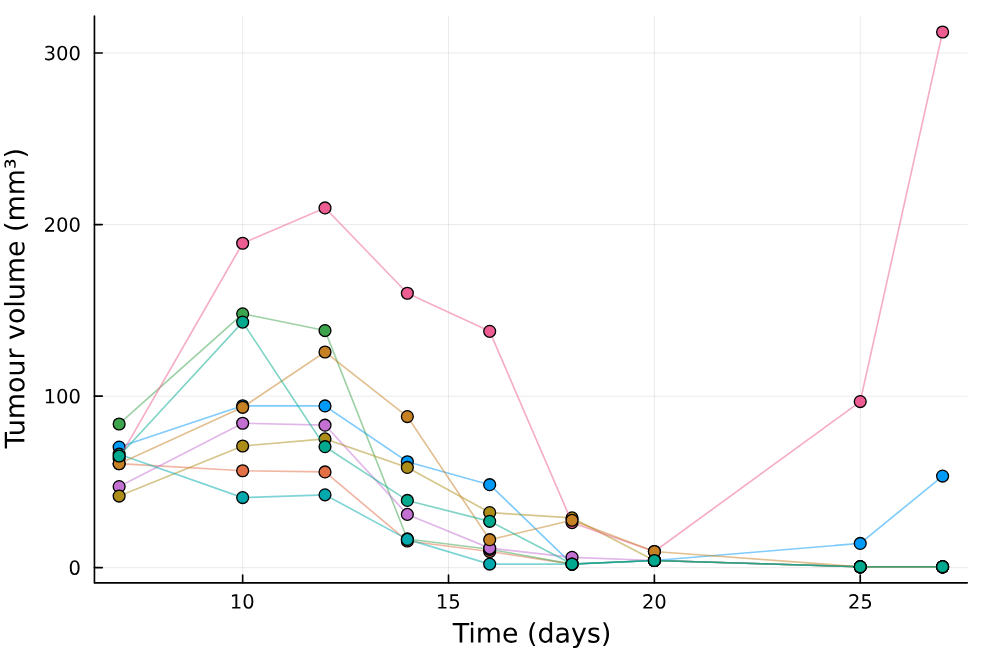
\includegraphics[scale=0.3]{crnoncr3.png}
    \caption{Evolution of tumour volume over time for a batch of mice shows that they present two distinct behavours: CR or non-CR (each trace is an individual mouse)}
    \label{fig:outcomedual}
\end{figure}

While these are promising results compared to alternative treatments for melanoma \cite{reviewImmunoMelanoma}, the heterogeneity of response (CR vs non-CR) could not be explained by the authors, and highlights the need to further analyse available data in order to identify the key biological parameters that can differentiate between CR and non-CR.

\subsection{Data Analysis with the Aid of Computational Modelling}\label{ssec:prevWork}

To have a better understanding of the immune response to CBD-IL-12, Dr Miyano, a previous member of the Tanaka group \cite{takuya}, proposed to use a computational modelling approach. Computational models are common in pharmacodynamics as they can be analysed with mathematical tools, potentially revealing key mechanisms to optimise the treatment while minimising the number of animal tests. He developped a mechanistic model (Fig.~\ref{fig:mech}b) based on our current model of the immune processes outlined in Section~\ref{sec:cancer} (see Fig.~\ref{fig:mech}a). This mechanistic model can predict tumour growth given a treatment, along with the concentration of IFN$\gamma$, CBD$^+$ and PD-1. The meaning of each model parameter is shown in Appendix~\ref{app}. It must be noted that this mechanistic model was developed to accomodate for different treament regimen, including combination therapy (CBD-IL-12 with checkpoint inhibitor drugs, called CPI). This is indicated by the two green boxes on Fig.~\ref{fig:mech}b, which indicates the presence of their respective drug. Since we are only concerned with monotherapy in this project, the CPI box can safely be ignored.
\begin{figure}[!ht]
    \centering
    \begin{subfigure}{.49\textwidth}
        \centering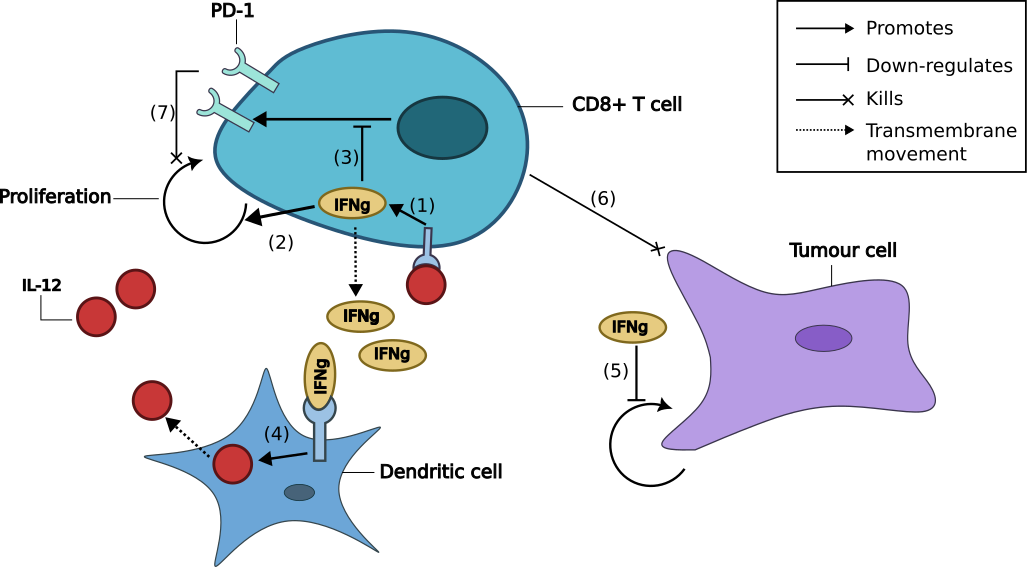
\includegraphics[scale=0.3]{finalBM.png}
        \caption{}        
    \end{subfigure}
    \begin{subfigure}{.49\textwidth}
        \centering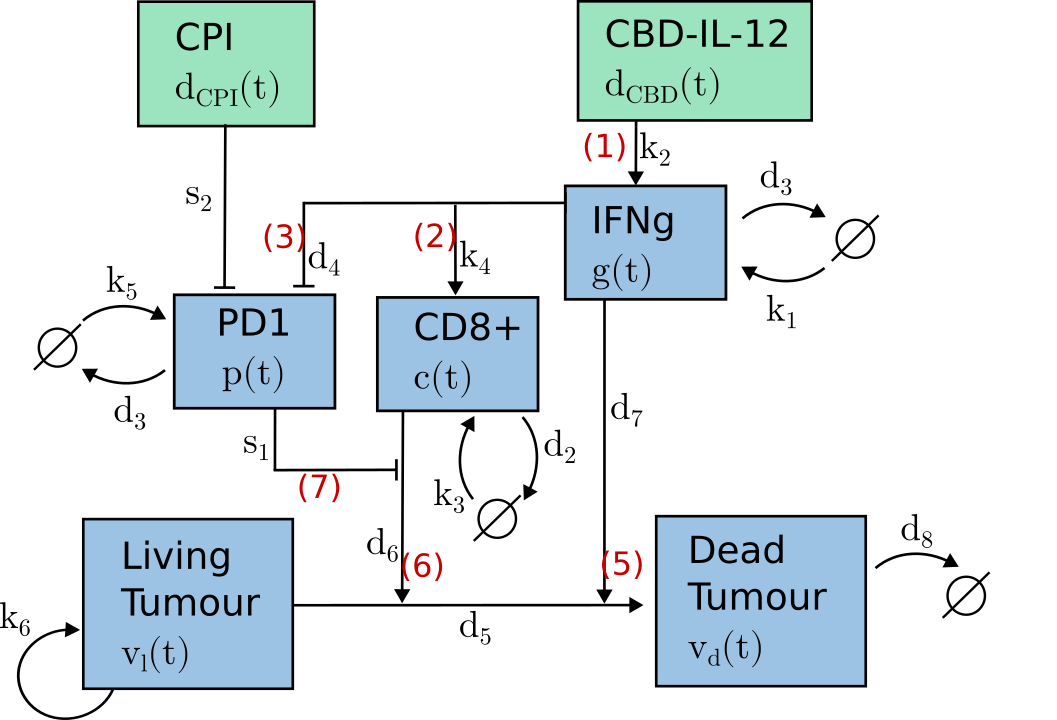
\includegraphics[scale=0.3]{finalCP.png}    
        \caption{}
    \end{subfigure}
    \caption{Mechanistic model of the IL-12-enhanced immune response. Numbers in the figures are to identify corresponding processes. \\
    \textbf{(a)} Illustration of the action mechanisms of IL-12-based cytokine (such as CBD-IL-12). Processus included in the model are: (1) IL-12-induced production of IFN$\gamma$ by T-cells, (2) upregulation of CD8$^+$ T-cells proliferation by IFN$\gamma$, (3) down-regulation of the PD-1 immunosuppressive pathway, (4) IFN$\gamma$-triggered production of IL-12 by dendritic cells, (5) reduced proliferation of tumour cells through suppressed angiogenesis and (6) CD8$^+$-mediated cytotoxic activity.\\
    \textbf{(b)} Diagram of the molecular interactions in the tumour microenvironment. Green boxes represent the inputs (drugs), which are fixed since we consider a specific treatment regimen (see Section~\ref{ssec:cbd}). Blue boxes represent the five state variables. All kinetic rates, corresponding to model parameters, are shown next to the corresponding process. Note that the IFN$\gamma$-priming process is missing, as the current mechanistic model does not include the feedback loop.}
    \label{fig:mech}
\end{figure}

This model can be represented by the following set of Delay-Differential Equations (DDEs) \cite{takuya} (see Fig.~\ref{fig:mech}b and Appendix~\ref{app} for the explanation of each symbol): 
\begin{align*}
    \dot{g}(t) &= k_1 + k_2 [d_{CBD}(t) + d_{12}(t)] - d_1g(t) \\ 
    \dot{c}(t,t-t_d) &= k_3 + k_4g(t-t_d)-d_2c(t) \\ 
    \dot{p}(t) &= k_5 - [d_3 + d_4g(t)]p(t) \\ 
    \dot{v}_l(t) &= k_6\left[1 - \frac{v(t)}{v_{max}} \right]v_l(t) - \left[d_5 + \frac{\frac{d_6c(t)}{1+s_1p(t)(1-d_{CPI}(t))}+d_7g(t)}{1+s_2v(t)}\right]v_l(t)\\
    \dot{v}_d(t) &= \left[d_5 + \frac{\frac{d_6c(t)}{1+s_1p(t)(1-d_{CPI}(t))}+d_7g(t)}{1+s_2v(t)}\right]v_l(t) - d_8 v_d(t)
\end{align*}

The parameters of this mechanistic model all represent biological factors that could potentially be responsible for the diverging treatment outcomes. However, these parameters are kinetic rates that cannot be measured experimentally: they can only be estimated from observable data (which is tumour volume in our project): this is called parameter estimation. However, when performing parameter estimation on multiple time series, one must choose the pooling type, which relates the different time series together. In the context of this project, where each time series correspond to an individual mouse, no-pooling means that each mouse is considered independently. Parameter estimation is thu performed on each mouse seperately. On the other hand, complete-pooling assumes that the parameters are completely homogeneous accross the experients (i.e., all time series are characterised by the same parameter combination). It is performed by averaging all time series together, resulting in one unique average behaviour. 

Hines, another previous member of the Tanaka group, applied parameter estimation on the mechanistic model by assuming complete-pooling. He obtained a set of parameters that can parameterise the mechanistic model so that it reproduces the average growth curve. However, the shortcoming of the complete-pooling approach is that it completely ignores the heterogeneity between individual and assumes that all individual behaves the same. It hence cannot to explain the heterogeneity of outcomes. This motivates us to use alternative pooling methods that could help us identify the key biological factors that differentiate between CR and non-CR.

Additionally, Hines noted that a key element that could explain why some mice exhibited continued immune response tens of days after the treatment was injected, thus achieving CR, could be a positive feedback loop that causes sustained production of IL-12, even days after injection. This is motivated by findings that positive feedback loops in cellular signalling systems can lead to switch-like behaviour \cite{bistable}. In such systems, a short-lived input can have a long-lasting impact on the steady state, even when it is removed. While a positive feedback loop is not present in the current mechanistic model, Hines identified a biologial process (IFN$\gamma$ priming, see \ref{sec:cancer}) corresponding to a positive feedback loop that could potentially be added to the model.

% This process, called parameter estimation, was investigated by Hines, another previous member of the Tanaka group. However, naive parameter estimation can only work to extract parameter from one single time series, and hence cannot be directly applied to the collection of times series obtained by the lab. Hines' approach was to fit the mechanistic model to the average growth curve. This resulted in a set of parameters that can explain (i.e., reproduce) this average behaviour. However, Hines concluded in his report that this set of parameter was not sufficient to help differentiating the different drug responses, as it can only reproduce an average curve that in essence represents neither a CR outcome nor a non-CR outcome. Additionally, he also mentioned that a key biological process, the IFN$\gamma$-priming feedback loop, was missing from the mechanistic model, which could potentially impact its accuracy and reliability.

% Hines' conclusion motivates us to use alternative parameter estimation methods that could help us identify the key biological factors that differentiate between CR and non-CR, by taking into account the whole dataset obtained in the lab.

\subsection{Proposed Approach: Hierarchical Bayesian Modelling}

An alternative parameter estimation technique that we propose to use is Bayesian modelling, which comes with two advantages crucial to solve the issue outlined by Hines:
\begin{enumerate}
    \item Unlike the parameter estimation used by Hines, Bayesian approach do not provide point estimate for each parameter, but rather probability distributions. Distributions, compared to point estimate, contain additional information that could help us understand which mechanisms drive the immune response and the complete response rate. One possible way distributions can be useful is outlined in \cite{toniPHD}: they allow us, in the case of parameter estimation, to quantify the sensitivity of the model to each parameter. For a given distribution associated to a parameter, a narrow credible interval (CI) means that the model is sensitive to this parameter. The opposite is true for a wide credible interval.  
    \item Bayesian modelling allow us to perform partial-pooling, which is a combination of no-pooling and complete-pooling. It formulates that, for a set of time series, each time series (and their corresponding estimated parameter set) are not completely independent nor homogeneous from each other, but rather contain some shared information and some individual variability. This is called hierarchical Bayesian modelling.
\end{enumerate}

\section{Aims and Objectives}
\noindent The aim of the project is to identify the key biological parameters responsible for the different outcomes observed in the lab (CR vs non-CR)\\[8pt]
\textbf{Objective 1:} develop a hierarchical Bayesian model based the mechanistic model that can reproduce the experimental data.\\ 
\textbf{Objective 2:} compute the probability distributions of the model parameters and verify whether they are bimodally distributed (to explain the two outcomes).\\ 
\textbf{Objective 3:} evaluate the impact of the IFN$\gamma$ priming pathway on the treatment outcome. 

\section{Ethical Analysis}

Treatments and experiments on the specimens used, mice in this case, were approved by the Institutional Animal Care and Use Committee of the Univerity of Chicago (see Methods section of \cite{cbdil12}).

The data derived from these experiments holds potential for understanding treatment response in cancer, aiding in the optimization of therapies for human use. Long-term implications involve the potential for groundbreaking advancements in cancer treatment, benefiting society globally. As this concerns development of drugs for human use, it is necessary to develop a robust work ethics that avoid developing harmful therapies to human. Thus, to ensure that the results are reliable and can be reproduced by anyone, the full analysis along with the code will be published on GitHub.

\section{Literature Review on Bayesian Parameter Estimation}\label{sec:littrev}

As mentioned in Section~\ref{sec:specs}, the project requires a parameter estimation method that can be applied to mixed-effects models. In this section, we first give a more rigorous definition of the parameter estimation along with an overview of the different methods available. We then review a specific method, called hierarchical Bayesian modelling, and highlight its particular relavance to the project. 

\subsection{Definition and Notation}
Let the general definition of a DDE model be: 

\begin{align*}
    \diff{X_i}{t} = f_i(t, \boldsymbol{X}(t), \boldsymbol{X}(t-\tau)| \boldsymbol{\theta}), \qquad t \in [t_0, t_{max}], i = 1, \ldots, I
\end{align*}

where $\tau$ denotes a constant delay, so that the rate of change of state $X_i$ depends on both the present state $\boldsymbol{X}(t)$ and a past state $\boldsymbol{X}(t-\tau)$. The subscript \textit{i} indexes the different state variables of interest, and $\boldsymbol{\theta}$ is the (unknown) vector of the parameters for the DDE model. This parameter vector is different for each treated mouse, as it uniquely characterises its treatement response, and hence we denote with $\boldsymbol{\theta}_j$ the parameter vector that characterises the $j$-th mouse. The experimentally observed tumour evolution for the $j$-th mouse is denoted by $\boldsymbol{y}_j$, and each of its elements is the tumour volume observed at a given time, noted $y_{j}(t)$. The aim of parameter estimation is to retrieve the parameter vector $\boldsymbol{\theta}_j$ that can reproduce the observed data $\boldsymbol{y}_j$. 

% Many statistical approaches have been developed to perform parameter estimation on differential equation models from noisy data \cite{liu_wang}. However, most of them cannot be applied to mixed-effect models. In the context of pharmacodynamics model , Donnet et al, 2013 \cite{revParamEst} reviewed different techniques available to perform parameter estimation. While many For analysis of population data with observational noise, only two methods are available: Expectation-Maximisation (either Stochastic \cite{SAEM} or using First-Order Condition \cite{foce}) and Bayesian parameter estimation \cite{rosenbaum}. The authors concluded that Bayesian modelling in particular is the most flexible method, since it does not rely on assumptions and hence work for both individual or population datasets, with or without noise, which is not the case for alternative methods. Additionally, it benefits from theoretical validity although at the cost of being more computationally intensive, whereas the First-Order Conditon method was not proven to always converge to the true posterior. Another relevant advantage is that Bayesian approach do not provide point estimate, but rather distributions, which could be key to explain outcome heterogeneity. Hence the Bayesian modelling approach seems to be the most relevant for the project. 

\subsection{Bayesian Parameter Estimation}

Bayesian Parameter Estimation is a method to estimate a parameter vector $\boldsymbol{\theta}$ given an observation vector $\boldsymbol{y}$. Contrary to frequentist approach, estimations are in the form of probability distributions (called posteriors, denoted $p(\boldsymbol{\theta}|\boldsymbol{y})$) rather than point estimates. 

For a situation where data about only one individual was gathered, the posterior distribution is defined as follows \cite{tbk_gelman}:
\begin{align*}
    p(\boldsymbol{\theta} | \boldsymbol{y}) \propto p(\boldsymbol{\theta})p(\boldsymbol{y}|\boldsymbol{\theta})
\end{align*} 
This formula is the direct application of Bayes' theorem. It is the product of the prior distribution $p(\boldsymbol{\theta})$, which represents our knowledge of the problem, and the likelihood $p(\boldsymbol{y} | \boldsymbol{\theta})$. Before further defining these distributions, we must extend this definition of the posterior distribution to work in situations where data about different individuals was collected. 
% To analyse such a type of problem, were dataset are not independent from each other, hierarchical Bayesian modelling is a common method \cite{revParamEst}\cite{rosenbaum}. For example, Rosenbaum et al., 2019 \cite{rosenbaum}, studied models of predator-prey systems, formulated as a set of ODEs, which display radically different behaviours depending on the values of certain kinetic rates that cannot be directly measured. By fitting times series of measurable data to a hierarchical Bayesian model, they could not only extract a specific set of parameters for each individual system; but also determine the regions in parameter space that led to radically different types of behaviour accross the population. This shows that hierarchical Bayesian modelling is a potent tool to explain heterogeneity in the dynamics of an ODE/DDE model by identifying the range of parameter values that lead to diverging outcomes. 

\subsection{Hierarchical Modelling}\label{sec:hierch}

In this project we seek to estimate a parameter vector $\boldsymbol{\theta}_j$ for each individual mouse $j$. However, as mentioned before, we model the data through partial-pooling: the parameter vectors $\boldsymbol{\theta}_j$ are connected in some way to each other, since they are all drawn from the same mice population. They way they are connected is as follows: in hierarchical Bayesian modelling, we can formulate that each $\boldsymbol{\theta}_j$ is sampled from a population-level distribution characterised by the (also unknown) hyperparameters $\boldsymbol{\phi}$. This common distribution corresponds to the shared information between each mouse, and the fact that each $\boldsymbol{\theta}_j$ is randomly sampled accounts for the individual variability. The objective is hence to find the distribution of both $\boldsymbol{\theta}_j~\forall j$ and $\boldsymbol{\phi}$. The Bayesian parameter estimation framework integrates this additional assumption by changing the posterior to \cite{tbk_gelman}:
\begin{align*}
    p(\boldsymbol{\theta}_j, \boldsymbol{\phi} | \boldsymbol{y}) \propto p(\boldsymbol{\phi})p(\boldsymbol{\theta}_j|\boldsymbol{\phi})p(\boldsymbol{y}|\boldsymbol{\theta}_j)
\end{align*} 

This expression is a product of the hyperprior $p(\boldsymbol{\phi})$, the population distribution $p(\boldsymbol{\theta}_j|\boldsymbol{\phi})$ and the likelihood $p(\boldsymbol{y}|\boldsymbol{\theta}_j)$.

\subsubsection{Hierarchical Priors and Hyperpriors}\label{sec:hierPriorsAndHyper}
In hierarchical Bayesian models, there are two types of parameters: hyperparameters $\boldsymbol{\phi}$ and individual parameters $\boldsymbol{\theta}_j$ \cite{tbk_gelman}. The key feature is that the simulated data is directly conditioned on the regular parameters, which are themselves drawn from population-level distributions characterised by hyperparameters. Hence, this results in two types of priors: hierarchical priors, that specify how to sample $\boldsymbol{\theta}$ using the hyperparameters $\boldsymbol{\phi}$; and hyperpriors that convery our knowledge about the potential values of~$\boldsymbol{\phi}$.

For the case of Bayesian parameter estimation on sets of time series, Rosenbaum et al, 2019 \cite{rosenbaum}, proposed to sample each ODE parameter from a Normal distribution. As Normal distribution are characterised by two values (mean $\mu$ and standard deviation $\sigma$), this resulted in two hyperparameters per ODE parameter. This can be summarised as follows, for a given scalar parameter $\theta$:
\begin{align*}
    \theta &\sim p(\theta | \phi) \Leftrightarrow \theta \sim \mathcal{N}(\phi_\mu, \phi_\sigma) \quad &&\textit{hierarchical prior} \\ 
    \phi_\mu &\sim p(\phi_\mu) \quad &&\textit{hyperprior for the hyper-mean} \\ 
    \phi_\mu &\sim p(\phi_\mu) \quad &&\textit{hyperprior for the hyper-standard deviation} 
\end{align*}

\subsubsection{Likelihood Function}
The likelihood describes the probability density of observing the data as a function of the parameters. In this case, it not only captures the dynamics of the mechanistic model, but also the observational noise. Typically, the mean of the obervations can be modelled as the solution of the DDE (parameterised by $\boldsymbol{\theta}_j$) and we can assume a white Gaussian observation error (with standard deviation $\sigma_\text{err}$)~\cite{liu_wang}\cite{likelihood_2}:
\begin{align*}
    \mathcal{L}(\boldsymbol{\theta}_j, \sigma_\text{err}) := p(\boldsymbol{y}_j | \boldsymbol{\theta}_j, \sigma_\text{err}) =  \prod_{t=t_0}^{t_{max}} \frac{1}{\sqrt{2\pi\sigma_\text{err}^2}} \exp\left(-\frac{(y_{j}(t) - Y_j(t|\boldsymbol{\theta}_j))^2}{2\sigma_\text{err}^2}\right),
\end{align*}
where t is the time and $Y_j(t|\boldsymbol{\theta}_j)$ is the solution of the DDE model parameterised by $\boldsymbol{\theta}_j$ (usually obtained by numerical methods). Without additional information about the measurement methods, this is the approach suggested by Rosenbaum et al \cite{rosenbaum}. 

It was also shown that, when the parameters to be estimated differ in value by several order of magnitude, fitting them on a logarithmic scale makes the inference more robut: faster convergence and more accurate posteriors \cite{rosenbaum}. This changes the likelihood function to the following:
\begin{align*}
    \mathcal{L}(\boldsymbol{\theta}_j, \sigma_\text{err}) = \prod_{t=t_0}^{t_{max}} \frac{1}{\sqrt{2\pi\sigma_\text{err}^2}} \exp\left(-\frac{(\ln[y_{j}(t)] - \ln[Y_j(t|\boldsymbol{\theta}_j)])^2}{2\sigma_\text{err}^2}\right),
\end{align*}

\subsection{Computational Methods}
While the previous section lays the theoretical background necessary to understand hierarchical Bayesian modelling, several issues can arise during practical implementation. In this section, we discuss two potential issues along with common solutions found in the literature.
\subsubsection{Numerical Approximation of Posterior Distributions}\label{sec:mcmc}
The posterior distribution $p(\boldsymbol{\theta}_j,\boldsymbol{\phi}|\boldsymbol{y}_j)$ represents the updated joint probability distribution for each parameter and hyperparameter, obtained by updating the priors with the likelihood function through the Bayes theorem. Ideally, the likelihood function can be written in closed-form, so that the posterior can be evaluated analytically as the normalised product between the priors and the likelihood (see Sec.~\ref{sec:hierch}).

However, in many cases the likelihood can only be evaluated for given a set of parameters, but its analytical form cannot be written. This can arise, as in this project, when it relies on a set of differential equations that can only be solved numerically. In these cases, a common approach is to use Markov Chain Monte-Carlo (MCMC) \cite{mcmcTuto}. MCMC is a method used to estimate a probability distribution when we only know how to calculate the probability density function for a given sample of the parameter space. In Bayesian modelling, it approximates the posterior by iteratively sampling random sets of parameters and calculting their corresponding posterior probability. This set of samples is called a MCMC chain. As its length grows to infinity, the distribution approximated through MCMC converges toward to true distribution. 

Several metric exist to measure convergence of the MCMC chains, a key characteric as it reflects the quality of the approximation of the distribution \cite{moins2023use} (in this case, of the posterior distribution). The most popular method to assess convergence is the potential scale factor reduction, usually termed $\hat{R}$, developed by Gelman et al., 1992 \cite{rhat}. It can be calculated as follows:
\begin{align*}
    \hat{R} &= \frac{m+1}{m}\frac{\hat{\sigma}^2_+}{W}-\frac{n-1}{mn} \\ 
    W &= \frac{1}{m(n-1)}\sum^m_{j=1}\sum^n_{t=1}(\psi_{jt}-\bar{\psi}_j)^2 
\end{align*}
Where $m$ is the number of chains used to explore the posterior in parallel, $n$ is their length, $\hat{\sigma}^2_+$ is the variance of the chain with the highest variance, $\psi_{jt}$ is the value of the $j$-th chain at the $t$-th iteration, and $\bar{\psi}_j$ the mean value of the $j$-th chain. The authors additional highlight that a value close to 1 usually indicates convergence, usually the criterion is $\hat{R}<1.05$ for convergence.

\subsubsection{Reduction of the Parameter Space through Sensitivity Analysis}
As Bayesian parameter estimation is computationally intensive  \cite{revParamEst}, this approach can benefit, in terms of compution time, from reducing the number of parameters when possible. Varella et al, 2012 \cite{varellaEFAT}, proposed a method to reduce the number of parameters in ODE models through sensitivity analysis. By taking the example of a crop growth model (the STICS model) with 13 parameters, the authors used an eFAST sensitivity analysis to determine the total sensitivity index ST for each parameter. This index indicates the fraction of the variance of model output variable that is imputable to a given parameter and its interaction with other parameters. For a parameter vector $\boldsymbol{\theta}$, the ST index of the $i$-th parameter can be computed as follows:
\begin{align*}
    ST_i =\frac{ V(Y) - \sum_{j \neq i}V_j}{V(Y)},
\end{align*}
where $Y$ is the model output variable, $V(Y)$ is its total variance and $V_j$ is the variance of Y when only $\boldsymbol{\theta}_j$ is varied.
The authors proposed to use this metric to classify parameters into two categories: if ST$>$0.1, the corresponding parameter should be retained and considered as a free parameter. Otherwise, the parameter can be fixed to a nominal value, found in the literature for example. 

Vazquez-Cruz et al, 2014 \cite{tomgro}, applied this method to another crop model called TOMGRO. After reducing the number of parameters from 17 to 8 (using the screening technique explained above), they showed that the reduced model was still able to reproduce experimental data with level of error comparable to the full model.  

\section{Risk Register}
The risks associated with the project along with a mitigation plan are described in Table~\ref{tbl:hyperparams}

\begin{table}[!ht]
    \caption{Table of the different risks associated with the project's objectives}

    \label{tbl:hyperparams}
\begin{longtable}{|p{3.5cm}|p{2.3cm}|p{2.3cm}|p{8cm}|}
    \hline
    \textbf{Risk} & \textbf{Likelihood} & \textbf{Impact} & \textbf{Mitigation Strategy}\\
    \hline
    \endfirsthead
    \hline
    \textbf{Risk} & \textbf{Likelihood} & \textbf{Impact} & \textbf{Mitigatio Strategy}\\
    \hline
    \endhead
    \hline
    \multicolumn{4}{|r|}{\textit{Continued on next page}} \\
    \hline
    \endfoot
    \hline
\endlastfoot
        \hline
        MCMC chains do\newline not converge  & High & Very high & 
        Two alternative methods can be used in this case.
        \textbf{Approximate Bayesian Computations,} which is a approach that does not rely on a likelihood function. It is relatively easy to implement but introduces additional approximation error. \textbf{Model simplification}, an approach proposed in \cite{gelman2020bayesian}. It consists of simplifying the likelihood function, and does not introduce additional error.
        \\ \hline 
        Model does not\newline pass validation protocol& High & Very high & Modify the immune response model to ensure that all key interactions are translated in the mechanistic model. We especially plan to implement the positive feedback loop mentioned in Section~\ref{ssec:prevWork}. \\ \hline 
\end{longtable}
\end{table}
\section{Evaluation}\label{sec:eval}
\textit{Objective 1: Bayesian Model}\\[3pt]
    The first objective of the project is to design a hierarchical Bayesian model. Once it is built, we must first verify its validity before proceeding to the next objective . We will follow the validation procedure outlined in \cite{gelman2020bayesian}. It consists of three tests that must each be passed:
\begin{itemize}
    \item \textbf{Prior Predictive Check:} we sample 1,000 sets of parameter from the priors and simulate tumour growth for each of them. The 95\% credible interval of the resulting collection of time series should contain our expected range of curves we can expect, otherwise the test is not passed.
    \item \textbf{Fake Data Check:} to perform this test, we first need to generate a artificial dataset using known values of parameters, and then fit the Bayesian model to these fake datasets. If the 95\% credible interval of the posterior distributions each include the corresponding true parameter value, then the model passes the test. Additionally, to ensure that the posterior distributions are reliable, we must verify that the MCMC chains converge (otherwise, it means that we cannot make inference from the posteriors). Their corresponding $\hat{R}$ must be below 1.05 (see Sec.~\ref{sec:mcmc})
    \item \textbf{Posterior Predictive Check:} this is analogous to the prior predictive check, except that parameter are drawn from the marginal posterior distributions instead of the prior distributions. This results in a collection of simulated time series. The criterion for the model to pass the test is that the 95\% credible interval should contain the experimental time series obtined in the lab. 
\end{itemize}
% \textit{Convergence of the MCMC Chains}\\[3pt]
% As mentioned above, convergence of the MCMC chains is a critical element that needs to be evaluated, as it reflects the quality of the approximation of the posterior distribution \cite{moins2023use}. The most popular method to assess convergence is the potential scale factor reduction, usually termed $\hat{R}$, developed by Gelman et al., 1992 \cite{rhat}. It can be calculated as follows:
% \begin{align*}
%     \hat{R} &= \frac{m+1}{m}\frac{\hat{\sigma}^2_+}{W}-\frac{n-1}{mn} \\ 
%     W &= \frac{1}{m(n-1)}\sum^m_{j=1}\sum^n_{t=1}(\psi_{jt}-\bar{\psi}_j)^2 
% \end{align*}
% Where $m$ is the number of chains used to explore the posterior in parallel, $n$ is their length, $\hat{\sigma}^2_+$ is the variance of the chain with the highest variance, $\psi_{jt}$ is the value of the $j$-th chain at the $t$-th iteration, and $\bar{\psi}_j$ the mean value of the $j$-th chain. The authors additional highlight that a value close to 1 usually indicates convergence, usually the criterion is $\hat{R}<1.05$ for convergence.

\textit{Objective 2: Bimodal Distributions for the Parameters}\\[3pt]
Once the Bayesian model has been validated, we can use it to compute the posterior distributions for each parameter. To identify the key parameters that can differentiate between CR and non-CR, along with their threshold value that seperate each outcome, we propose the following method:
(1) We label each experimental time series as either CR or non-CR (depending on whether tumour volume converged to 0 or diverged at the end of the experient). We can then construct two distinct datasets: one containing only CR time series, and one with only non-CR time series.
(2) We fit the model to each dataset seperately. We hence obtained two sets of posterior distributions, each corresponding to a population that either achieved CR or non-CR, respectively. For any parameter, if the CR-population has a statistically different hypermean from the non-CR-population, we can conclude that this parameter is differently distributed between mice that achieved CR and those who did not. 
(3) By identify all parameters that are differently distributed between the two populations, we can construct a set of biological parameters that help us differentiate between CR and non-CR (we call this set the responder profile). If this set is non-empty, it means that the project was successful, and subsequent animal experiments can potentially be undertook to verify these results.
% For objective 2, through the validated Bayesian model we will (1) identify the parameters that can differentiate responders from non-responders; (2) define the range of values of each of the parameters to differentiate CR from partial responders and non responders. To do so, we will compute the posterior distribution of the hypermean of each parameter for two datasets: one with only time series corresponding to CR, and one with only non-CR time series. If the mean of the posterior distributions are distinct (they are not within the 95\% credible interval of each other), we can conclude that the Bayesian model can successfully help us differentiating between CR and non-CR. The parameters for which the  by identifying the key biological factors. Potential future work would be to identify one or more biomarkers, e.g., PD-1, whose presence and/or its concentrations at given timepoints post intervention can reflect the responder profile parameters, hence has predictive value for future studies.

\textit{Objective 3: Impact of IFN$\gamma$ priming}\\[3pt]
To evaluate the impact of the IFN$\gamma$ priming positive feedback loop, we will first modify the Bayesian to include it. Once it has been validated following the same procedure as highlighted above (see Sec.~\ref{sec:eval} for Objective 1), we will construct a new responder profile and compare it with the previously obtained profile (that does not include the feedback loop).

\section{Preliminary Results}

\subsection{Verifying the Dynamics of the Mechanistic Model}\label{sec:montecarloSA}

Before extending the mechanistic model to a Bayesian model (objective 1), the very first aspect of the mechanistic model that we wanted to verify was its ability to capture two specific treatment outcome: CR vs non-CR. The is a necessary feature whithout which we would not be enable to differentiate between the different outcomes observed in the lab. As these behaviours can essentially be characterised by the fixed-points of the model (if the steady-state behaviour of the model converges to high values of tumour volume, it is a non-CR behaviour, and vice-versa). We opted for a grid-search stability analysis, meaning that we sample reguarly-spaced points in parameter space and classify them as either CR or non-CR. The choice of this method was motivated by the fact that this method is fast to implement compared to finding the fixed points numerically. Its shortcoming is that it can only find an approximation of the bifurcation boundary, but this does not matter for this step since the goal was to simply to check the existence of a clear boundary rather that its exact location. To avoid sampling in a 21-dimensional parameter space, which would be too computationally heavy, we used Hines' findings, according to which the solution of the DDE model (i.e. the simulated tumour growth) is mostly sensitive to three parameters: $k_6$, $s_2$ and $d_1$ \cite{christian1}. Fig.~\ref{fig:mcsa} shows the resuls of this grid-search analysis, where each axis of the cube corresponds to the value of the parameter $k_6$, $s_2$ or $d_1$ respectively. Green dots represent a parameter combination which lead to CR (tumour volume below 10mm$^3$ at day 27), dots were colored in red otherwise. As can be seen, there seem to be a clear boundary between the two response modes, with very little ``mixing''. This suggests that it would be possible to predict how a given patient would respond to the treatment, by knowning on which side of the boundary he is.

\begin{figure}[!ht]
    \centering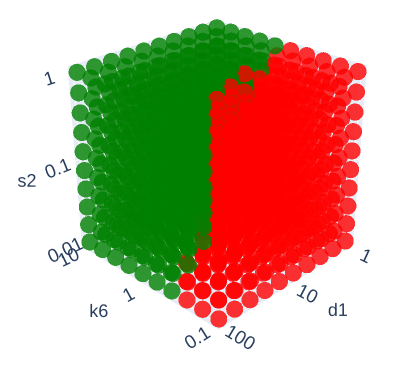
\includegraphics[scale=0.5]{stability.png}
    \caption{Grid-search stability analysis. Each dot represent a combination of parameters $k_6$, $d_1$ and $s_2$. Green indicates a combination that led to CR, red indicates non-CR. This shows that there is a clear boundary in parameter space between CR and non-CR}
    \label{fig:mcsa}
\end{figure}

\subsection{Construction and Validation of the Bayesian Model (Objective 1)}
In this section we show how our initial Bayesian model was tested, following the procedure highlighted in Section~\ref{sec:eval}. We focus on a reduced model with only three free parameters, $k_6$, $d_1$, $s_2$, as justified above (see Sec.~\ref{sec:montecarloSA}). All other parameters of the model were fixed to their respective value estimated by C. Hines through complete-pooling parameter estimation. This ensures that they do not bias the model towards an extreme outcome (whether CR or non-CR), since they characterise an ``average'' growth curve.

\subsubsection{Prior Predictive Check}
\textit{Note:} to represent a distribution truncated at 0, we use either a ``+'' (positive half) or ``-'' (negative half) superscript. For example: $X \sim  \text{Cauchy}^- \Rightarrow - \infty < X < 0$.

In this case, we do not have much data on the typical values of the parameters since it is impossible to measure it, so we aimed to design an uninformative prior. Fig.~\ref{fig:ppc_1} shows a plot of 1,000 tumour growth time-series. Each of them was simulated using a set of parameters drawn from the following prior distributions:
\begin{align*}
    \ln(k_6) \sim \text{Cauchy}^-(0, 1) \\ 
    \ln(d_1) \sim \text{Cauchy}^+(0, 1) \\ 
    \ln(s_2) \sim \text{Cauchy}^-(0, 1) \\ 
\end{align*} 
We chose Cauchy distributions since they are less informative than standard Gaussian distributions, allowing for values far from their center of mass. This is critical since we do not have much information about the true values of the parameters. In our priors, we assume that the parameters are log-Cauchy distributed to ensure that they are strictly positive, a necessary condition since they are biologial parameters. Additionally, the Cauchy distributions were truncated to ensure that the parameters are either below 1 (for $k_6$ and $s_2$) or above 1 (for $d_1$). This is to avoid numerical instability. [The threshold of 1 was chosen experimentally and needs to be refined more rigorously.]

Fig.~\ref{fig:ppc_1}, is the result of the prior predictive check. Each grey line represent a solution of the DDE model characterised by a random parameter combination sampled from the priors. The blue shade represents the 95\% credible interval, and the red line is the median growth curve. As we can see, the 95\% credible interval spans our expected range of curves (any curve between no growth and a continous growth up to 600mm$^3$), meaning that they are relatively uninformative priors. The median curve has the shape of the typical growth curve, as observed in the labs. Since the priors do not bias the model towards a CR or non-CR, but rather cover the full range of growth curve we might expect, we conclude that the prior predictive check is passed.
    \begin{figure}[!ht]
        \centering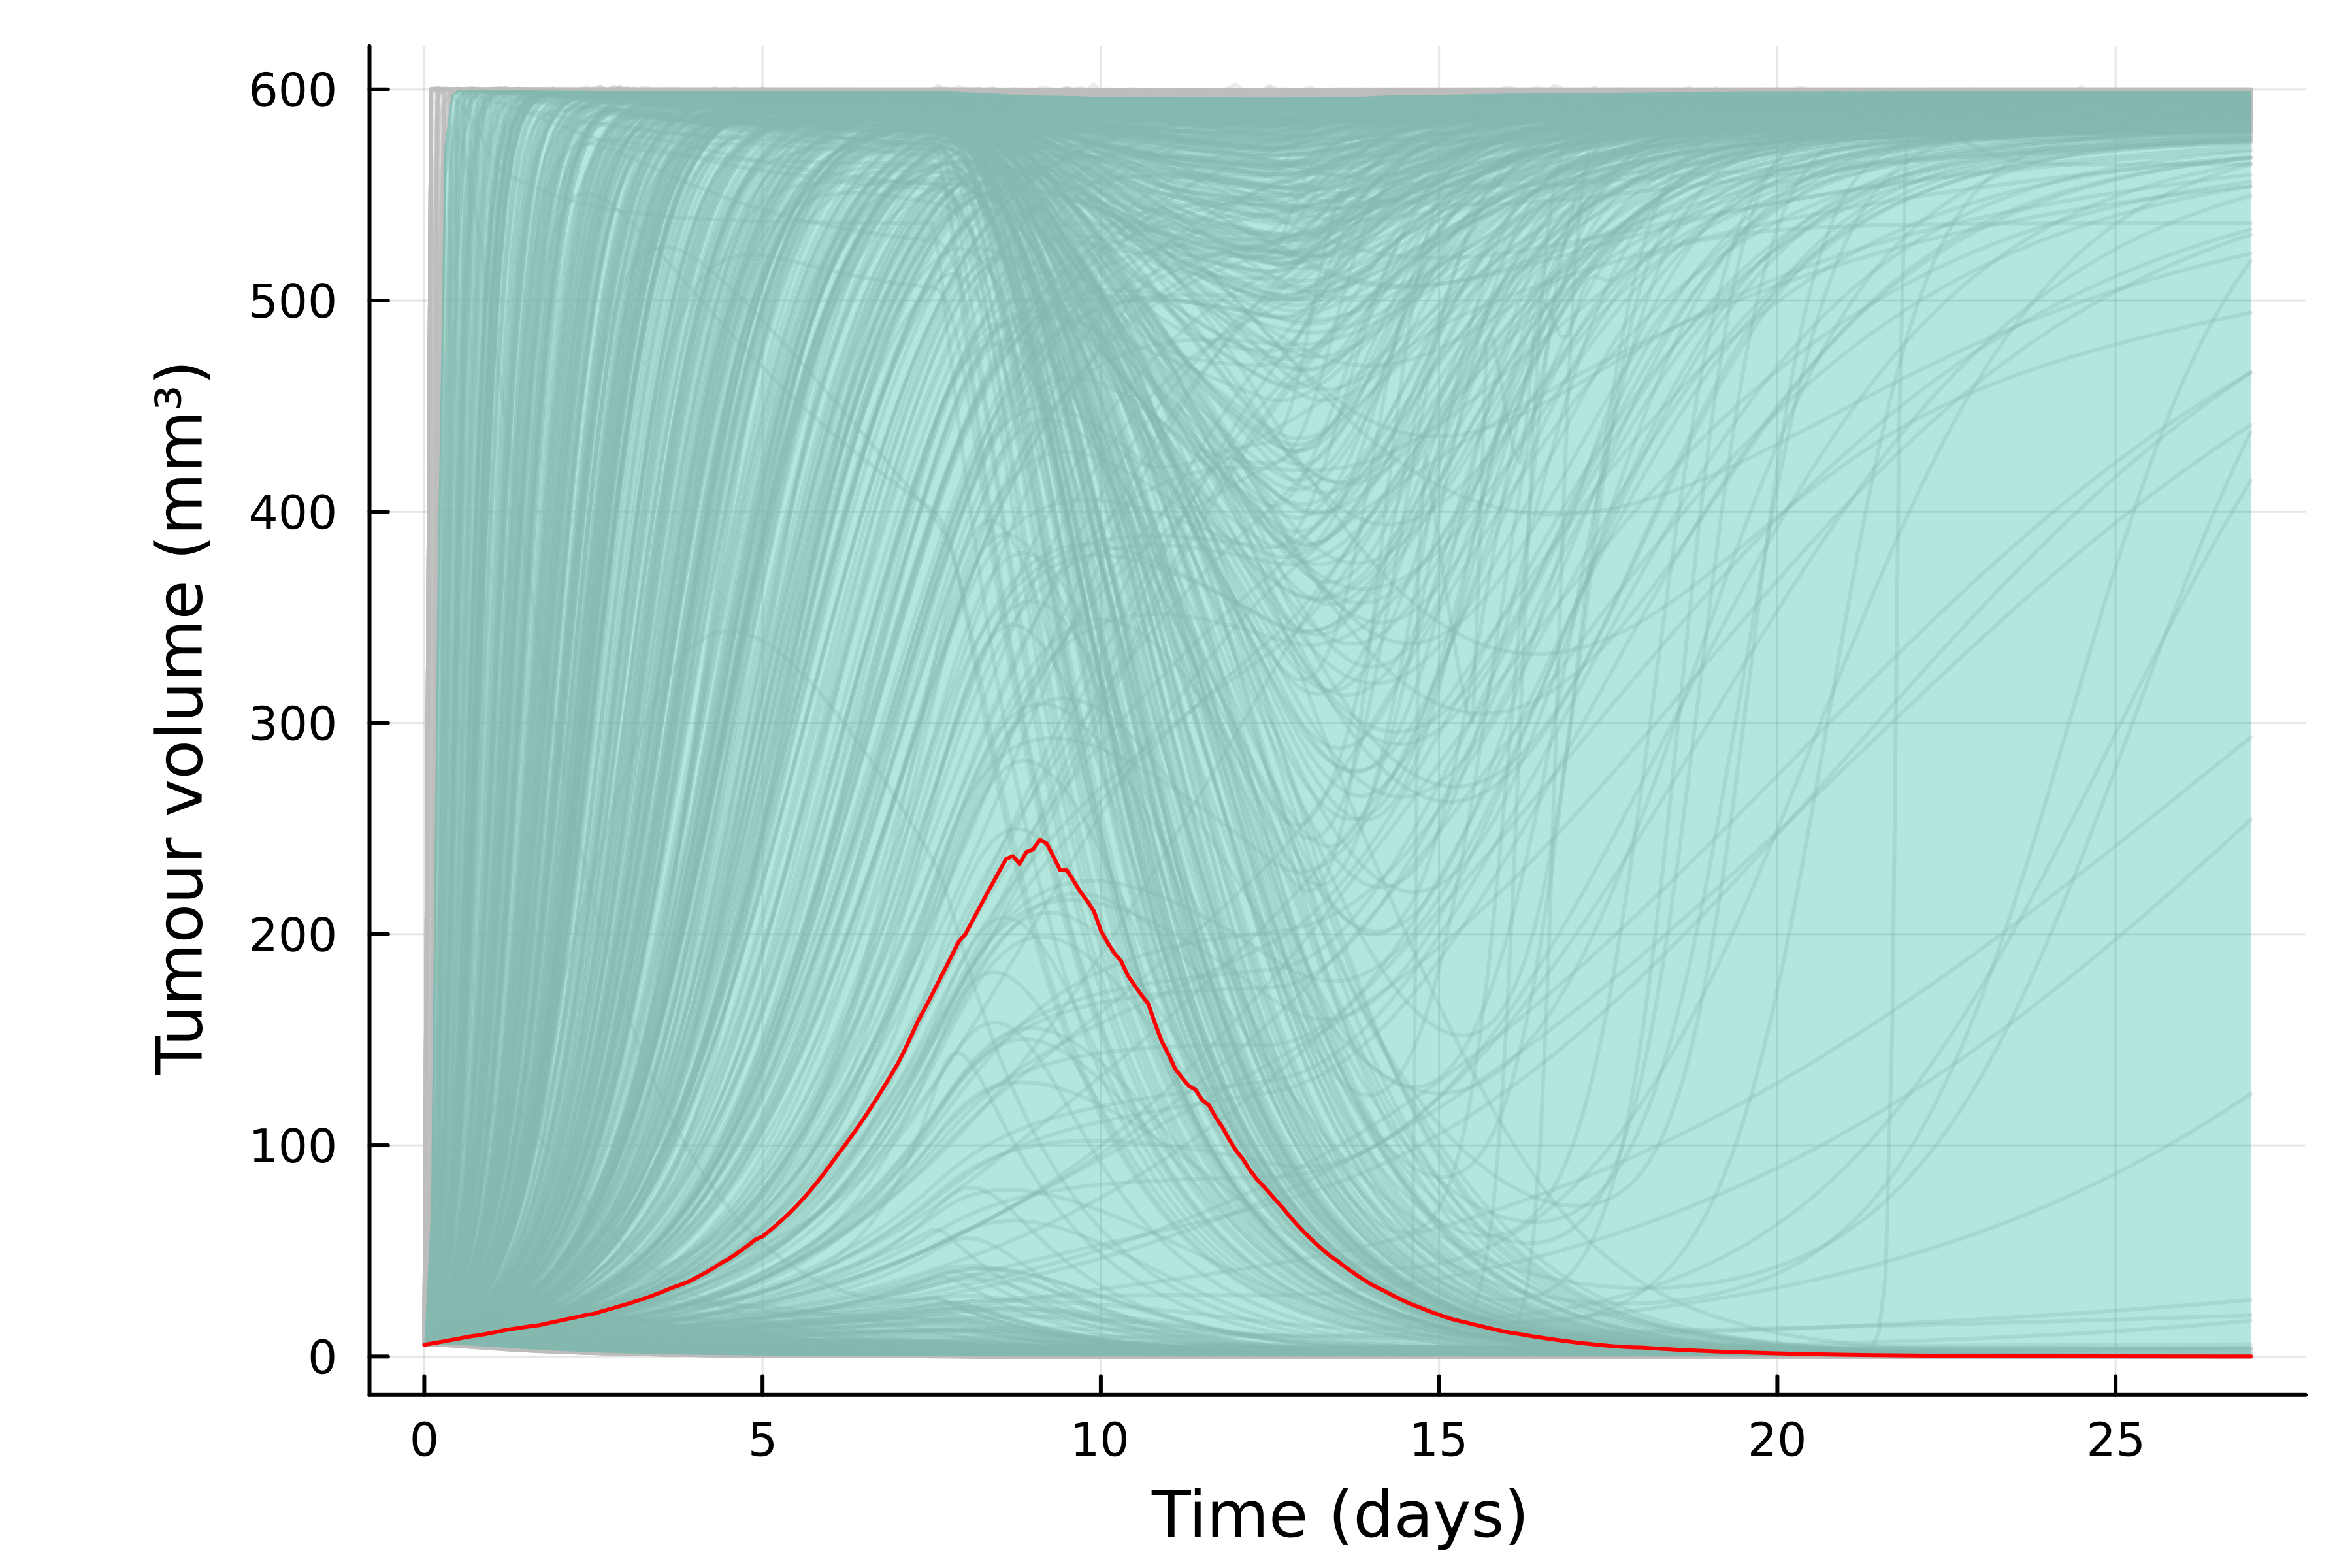
\includegraphics[scale=0.7]{LOGprout.png}
        \caption{DDE solutions (grey lines) for 1,000 parameter vectors $\boldsymbol{\theta}$ sampled from the priors. The 95\% credible interval for the tumour volume at each timestep (blue shade) shows that the model passes the prior predictive check: it contains our expected range of curves. The median grwoth curve (red line) confirms this, as it is very similary to the growth curve observed in the lab.}
        \label{fig:ppc_1}
    \end{figure}

% log10 y tumour growth 
% distinct instead of significant
% potential future work instead of aspirational outcome (due to time constraints)

\subsubsection{Fake Data Check}
For the fake data check, we first generate artificial datasets using known parameter values, and then fit the Bayesian model to these fake datasets. Comparing the estimated parameter value in the form of the posterior distribution to the true values can help us make informed decisions about modifying the model before proceeding to fit it to real data. While a successful fake data check (we can recover the true parameter values using the posteriors) does not mean the inference on real data will be successful or biologially meaningful, a failed fake data check implies that the model will never be able to fit on real data. In this case, the way the model fails can guide us when improving the model.

\textit{Data Generation}\\[5pt]
Each fake growth curve was generated by sampling a value of $\boldsymbol{\theta}$ from the prior distributions (shown in the previous subsection), and then simulating the tumour growth in the same way as for the prior predictive check. However, as biological data is always noisy, we also added some noise to make the fake dataset closer to what we would expect from the labs. This was done in two different ways, resulting in two distinct datasets. For dataset~A, we simply added a white Gaussian noise with variance $\sigma_\text{err}=1$ to the simulation (additive noise). The variance was chosen arbitraily, the only condition being that it is much smaller . than For dataset B, we added white noise to the log of the simulated curve (i.e. multiplicative noise). Using a standard Gaussian would result in too large noise values, so we chose a standard deviation of 0.3 to achieve similar levels of noise compared to dataset A. The generation process is summarized in Table~\ref{tbl:genproc}, where $x_*$ denotes a noiseless data point. The reason for using two different noise generation is that we observed, in the experimental data from the labs, that data points are usually more dispersed when they have a high value, suggesting an exponential relationship.\\ 
Additionally, each dataset contains 10 time series. Fig.~\ref{fig:fd_1} plots the fake data points against the original curve. For clarity, only 5 time series, selected at random, were shown.\\
\begin{table}[h!]
    \centering
    \caption{Summary of the generation process for the two datasets A and B}
    % \vspace{3pt}
    \begin{tabular}{c|c}
        \hline
        Dataset & Generation Process \\ \hline 
        A       & $x_A=x_*+\mathcal{N}(0,1)$ \\
        B       & $x_B=x_*\times e^{\mathcal{N}(0,\hspace{1.5px}0.3)}$ \\ \hline
    \end{tabular}
    \label{tbl:genproc}
\end{table}

\begin{figure}[!h]
    \centering
    \begin{subfigure}{.5\linewidth}
        \centering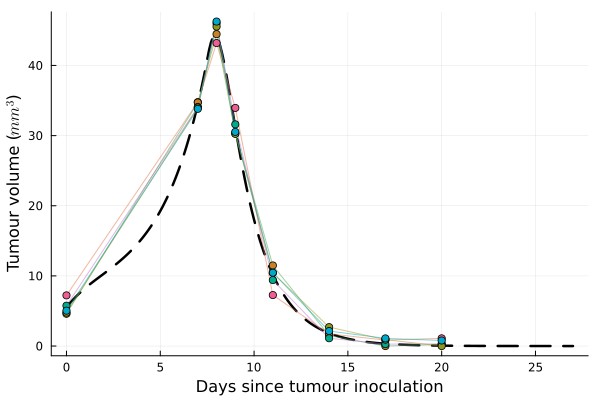
\includegraphics[scale=0.4]{model_validation/fd_1.png}
        \caption{Dataset A}
    \end{subfigure}%
    \begin{subfigure}{.5\linewidth}
        \centering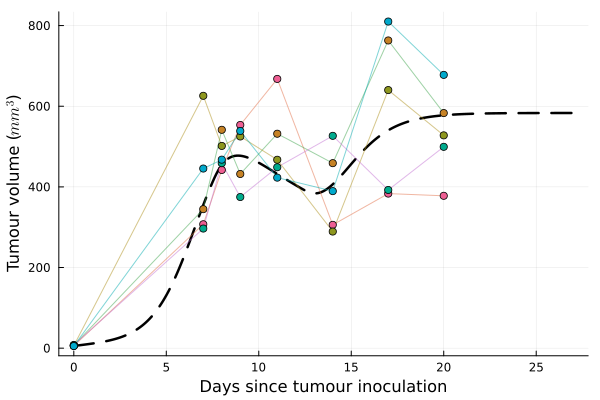
\includegraphics[scale=0.4]{model_validation/fd_2.png}
        \caption{Dataset B}
    \end{subfigure}
    \caption{Fake data sets (scatter plot and colored lines) generated from a baseline growth curve (dashed line), either with \textbf{(a)} additive noise or \textbf{(b)} multiplicative noise. Baseline curves were obtained by solving the DDE model parameterised by a vector $\boldsymbol{\theta}$ sampled from the prior distributions.}
    \label{fig:fd_1}
\end{figure}

\textit{Fitting the model to the fake datasets}\\[5pt] 
Before checking if the estimated values match the true ones, we first assess convergence of the MCMC chains. The $\hat{R}$ values (see Section~\ref{sec:eval}) are reported in Table.~\ref{tbl:rhat_2} as the average $\hat{R}$ value accross the 3 parameters. It must be noted that often, out of the 5 chains per inference, some chains  get trapped (assessed by visual inspection). In that case, they are excluded from the $\hat{R}$ calculation, and the ``Number of Chains'' column only repots the number of chains used to compute $\hat{R}$. If all chains are exlcuded, meaning that none of them converged, we simply report N/A.

\begin{table}[!h]
    \centering
    \caption{Assessement of convergence for the MCMC chains for uninformative priors}
    \begin{tabular}{c|c||c|c|c}
        \hline
        Data set & Pooling Type & $\hat{R}$ diagnostic & Number of Chains & Convergence  \\ \hline 
        \multirow{2}{*}{A}      & None     & 116.08 & N/A & No \\
                                & Complete & 298.67 & N/A & No \\ \hline 
        \multirow{2}{*}{B}      & None     & 1.092  & 3/5 & No \\
                                & Complete & 3.11   & N/A & No \\ \hline 
    \end{tabular}
    \label{tbl:rhat_2}
\end{table}
Looking at Table~\ref{tbl:rhat_2}, we can conclude that the chains did not converged, meaning that the model cannot make inference with $\boldsymbol{\theta} \in \mathbb{R}^3$ and uninformative priors. To further diagnose the model, we performed another set of inferences, except that the priors where highly informative:
\begin{align*}
    \ln(k_6) \sim \text{Cauchy}^-(\theta_{k_6}, 1) \\ 
    \ln(d_1) \sim \text{Cauchy}^+(\theta_{d_1}, 1) \\ 
    \ln(s_2) \sim \text{Cauchy}^-(\theta_{s_2}, 1) \\ 
\end{align*} 
where $\theta_x$ represent the true value of parameter $x$, used to generate the fake datasets. Convergence of this new set of inferences is shown in Table~\ref{tbl:rhat_3}. As we can see, convergence of the MCMC chains are still very poor, even with highly informative priors centered on the true parameter values.
\begin{table}[!h]
    \centering
    \caption{Assessement of convergence for the MCMC chains for informative Cauchy priors}
    \begin{tabular}{c|c||c|c|c}
        \hline
        Data set & Pooling Type & $\hat{R}$ diagnostic & Number of Chains & Convergence  \\ \hline 
        \multirow{2}{*}{A}      & None  & 18.15 & N/A & No \\
                                & Complete & 45.96 & N/A & No \\ \hline 
        \multirow{2}{*}{B}      & None  & 1.505 & 3/5 & No \\
                                & Complete & 1.014 & 2/5 & Yes \\ \hline 
    \end{tabular}
    \label{tbl:rhat_3}
\end{table}
\\[12pt]
It might be objected that Cauchy distributions are by definition not informative since a non-negligible portion of their mass stretches well beyond their standard deviation, contrary to normal distributions. This hence motivated us to perform one last fake data check, using the normal priors shown below to be even more informative: 
\begin{align*}
    \ln(k_6) \sim \mathcal{N}^-(\theta_{k_6}, 0.3) \\ 
    \ln(d_1) \sim \mathcal{N}^+(\theta_{d_1}, 0.3) \\ 
    \ln(s_2) \sim \mathcal{N}^-(\theta_{s_2}, 0.3) \\ 
\end{align*}
Convergence results are shown in Table.~\ref{tbl:rhat_4}. We can observe that chains converged or were close to convergence only for dataset B, showing that a log-normal transformation is key to make exploration of the posterior easier to perform.

\begin{table}[!h]
    \centering
    \caption{Assessement of convergence for the MCMC chains for informative Normal priors}
    \begin{tabular}{c|c||c|c|c}
        \hline
        Data set & Pooling Type & $\hat{R}$ diagnostic & Number of Chains & Convergence  \\ \hline 
        \multirow{2}{*}{A}      & None     & 7.387 & N/A & No \\
                                & Complete & 39.17 & N/A & No \\ \hline 
        \multirow{2}{*}{B}      & None     & 1.066 & 3/5 & Yes \\
                                & Complete & 1.111 & 5/5 & No \\ \hline 
    \end{tabular}
    \label{tbl:rhat_4}
\end{table}
~\\
\textit{Conclusion}\\[5pt]
Even with informative priors, the MCMC chains do not even converge. This suggests that the likelihood function is too difficult to explore and might contain discontinuities. As suggested by Gelman et al. (2020) in their \textit{Bayesian Workflow} document, the first step to take to address this issue would be to drastically simplify the likelihood function and re-assess performance of the model of fake datasets. Another approach that we are currently exploring would be to use Approximate Bayesian Computation. These two approaches will enable us to further diagnose the model to make appropriate corrections.


\section{Implementation Plan}\label{sec:plan}

\begin{figure}[!ht]
    \centering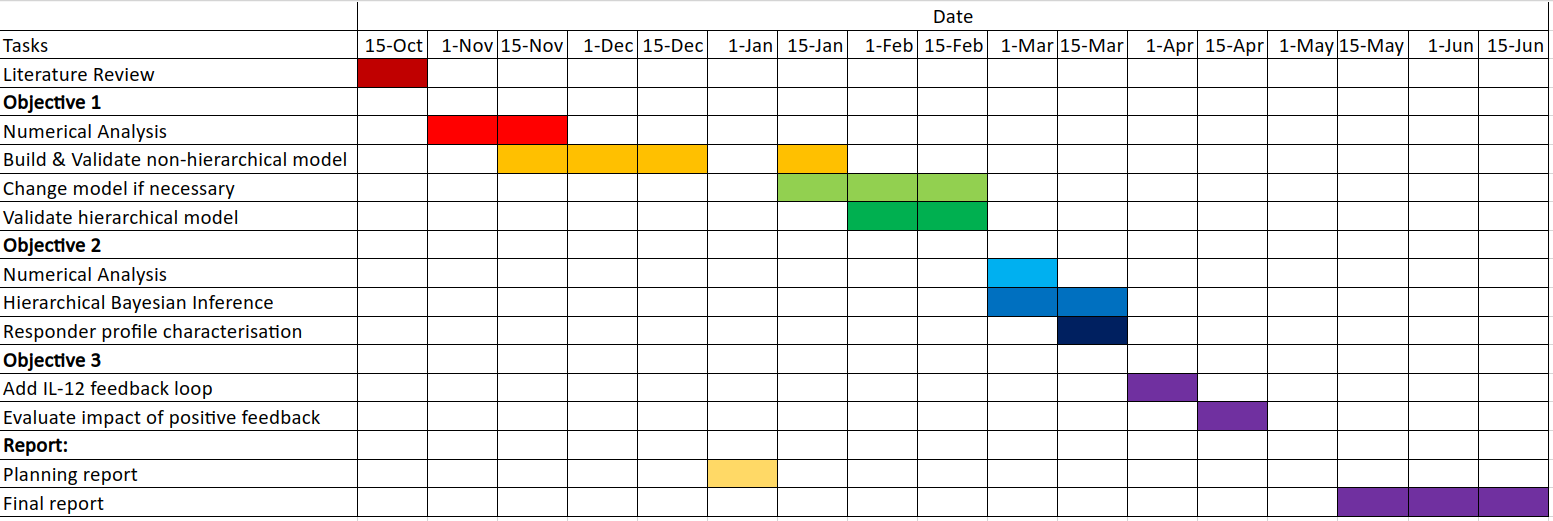
\includegraphics[scale=0.32]{testo.png}
\end{figure}

\clearpage
\newpage
\appendix
\section{Parameters of the Computational Model}\label{app}
\begin{table}[!h]
    \centering
    \caption{Parameters of Miyano's model along with their description}
    \begin{tabular}{c |l}
        \hline 
        Parameter & Description \\ \hline
        $t_{delay}$ & time delay from injection timiring to deliver CBD-IL-12 to tumour \\ 
        $t_{last}$ & time duration of drug effects of CBD-IL-12 \\ 
        $t_{delay12}$ & time delay from injection timing to deliver IL-12 to tumour \\
        $t_{last12}$ & time duration of drug effects of IL-12 \\ 
        $t_d$ & time delay for producing $CD8^+$ via IFN$\gamma$ \\ \hdashline
        $k_1$ & production rate of IFN$\gamma$ via unspecified pathways \\ 
        $k_2$ & production rate of IFN$\gamma$ via CBD-IL-12 \\ 
        $k_3$ & production rate pf CD8$^+$ via unspecified pathways \\ 
        $k_4$ & production rate of CD8$^+$ via IFN$\gamma$ \\ 
        $k_5$ & production rate of PD-1 via unspecified pathways \\ 
        $k_6$ & proliferation rate of tumour \\ \hdashline
        $d_1$ & elimination rate of IFN$\gamma$ via turnover \\
        $d_2$ & elimination rate of CD8$^+$ via turnover \\ 
        $d_3$ & elimination rate of PD-1 via turnover  \\ 
        $d_4$ & elimination rate of PD-1 via turnover IFN$\gamma$ \\ 
        $d_5$ & elimination rate of living tumour via turnover \\ 
        $d_6$ & elimination rate of living tumour via CD8$^+$ \\ 
        $d_7$ & elimination rate of living tumour via IFN$\gamma$ \\ 
        $d_8$ & elimination rate of dead tumour via turnover \\\hdashline
        $s_1$ & inhibition strength of PD-1 on anti-tumour effects of CDB$^+$ \\ 
        $s_2$ & inhibition strength of tumour volume on antitumour effects of IFN$\gamma$ and CD8$^+$ cells \\ \hline
    \end{tabular}
\end{table}

\clearpage
\newpage

\addcontentsline{toc}{section}{References}
\bibliographystyle{unsrt}
\bibliography{biblio}


\end{document} % This is the end of the document

%% Trash-city

% The goal of immunotherapy is to use a specific type of cytotoxic immune cells, the CD8$^+$ cells, to fight against cancer \cite{ReviewCPI}. As cancer can escape these killer cells through various mechanisms, this lead to a range of difference 

% While all cancer immunotherapies focus on using the natural immune system to fight against cancer, many different variations exist. The specific therapy of concern in this project is a combination of cytokine-based treatments and immune checkpoint inhibitors. Before explaining its specificities in more details, we will review the general principles behind the two aforementioned types of immunotherapy. In both case, a specific type of T-lymphocyte, the CD8$^+$ T-cells, is the central actor . CD8$^+$ differentiate itself from other T-cells through the expression of the membrane receptor CD8, and its main function is to directly carry out cytotoxic activity (i.e. killing the malignant cells) after detecting tumoural antigen~\cite{cd8Effects}.
%

% it is a pleiotropic molecule, meaning that it results in the release of numerous cytokines throughout the immune response~\cite{il12CytokineStorm}. One particular molecule released during this cytokine storm is the interferon-$\gamma$ (IFN$\gamma$). IFN$\gamma$ plays a dominant role within this cytokine storm, as not only does it have anti-angiogenesis effect~\cite{ifngAngiogenesis}, thus limiting cancer growth; but it also stimulate production Natural Killer cells \cite{ifngNKProd} (another type of cytotoxic cells capable of attacking tumours) and upregulate antigen-presenting pathways within tumour cells \cite{ifngAntigenExposure}. Finally, IL-12 facilitates T-cell proliferation by reducing negative regulatory pathways that lead to immunosuppression. Indeed, IL-12 inhibts the effect of the immune checkpoint PD-1, similarly to chekpoint inhibitors (CPI) treatments \cite{reducImmunoSuppression}. The more details mode of action is described in the following paragraph. [maybe need to mention trAEs? and poor performance so far...]
%
